%%%%%%%%%%%%%%%%%%%% author.tex %%%%%%%%%%%%%%%%%%%%%%%%%%%%%%%%%%%
%
%%%%%%%%%%%%%%%% Springer %%%%%%%%%%%%%%%%%%%%%%%%%%%%%%%%%%

\title*{A (nearly) full analysis of a GP run}
% Use \titlerunning{Short Title} for an abbreviated version of
% your contribution title if the original one is too long
\author{Nicholas Freitag McPhee, Maggie M. Casale, Thomas Helmuth and Lee Spector}
% Use \authorrunning{Short Title} for an abbreviated version of
% your contribution title if the original one is too long
\institute{Nicholas Freitag McPhee and Maggie M. Casale \at University of Minnesota, Morris; Morris, MN USA
\and Thomas Helmuth \at Washington and Lee University, Lexington, VA USA
\and Lee Spector \at Hampshire College, Amerherst, MA USA}

\maketitle

\abstract{We analyze the key events in a GP run!}

\begin{keywords}
	genetic programming, PushGP, ancestry graph, lineage, inheritance
\end{keywords}
\index{genetic programming}
\index{PushGP}
\index{ancestry graph}
\index{lineage}
\index{inheritance}
\\
\section{Introduction}
\label{sec:introduction}

Motivate the work!

\section{Plush genomes and PushGP operators}
\label{sec:background}

\todo{I'm hoping we can crib most of this section from previous works, e.g.,
	Tom's dissertation, the Plush GPTP paper, and other papers.}

We'll need to (quickly) outline the key elements of the Plush genome, including
the \texttt{:instruction} and \texttt{:close} components. (This run didn't use the
\texttt{:silent} component, so we can ignore that.)

We'll also need to describe the genetic operators used in PushGP/Clojush.

And replace-space-with-newline.

And simplification.

%Use the standard \verb|equation| environment to typeset your equations, e.g.
%%
%\begin{equation}
%a \times b = c\;,
%\end{equation}
%%
%however, for multiline equations we recommend to use the \verb|eqnarray| environment.
%\begin{eqnarray}
%a \times b = c \nonumber\\
%\vec{a}   \vec{b}=\vec{c}
%\label{eq:01}
%\end{eqnarray}

\section{Analysis of a run}

\begin{figure}[tb!p] %[b] sets the image at the bottom of the page; t = top, b = bottom, h = here%
	% \sidecaption
	% Use the relevant command for your figure-insertion program
	% to insert the figure file.
	% For example, with the graphicx style use
	\begin{center}
		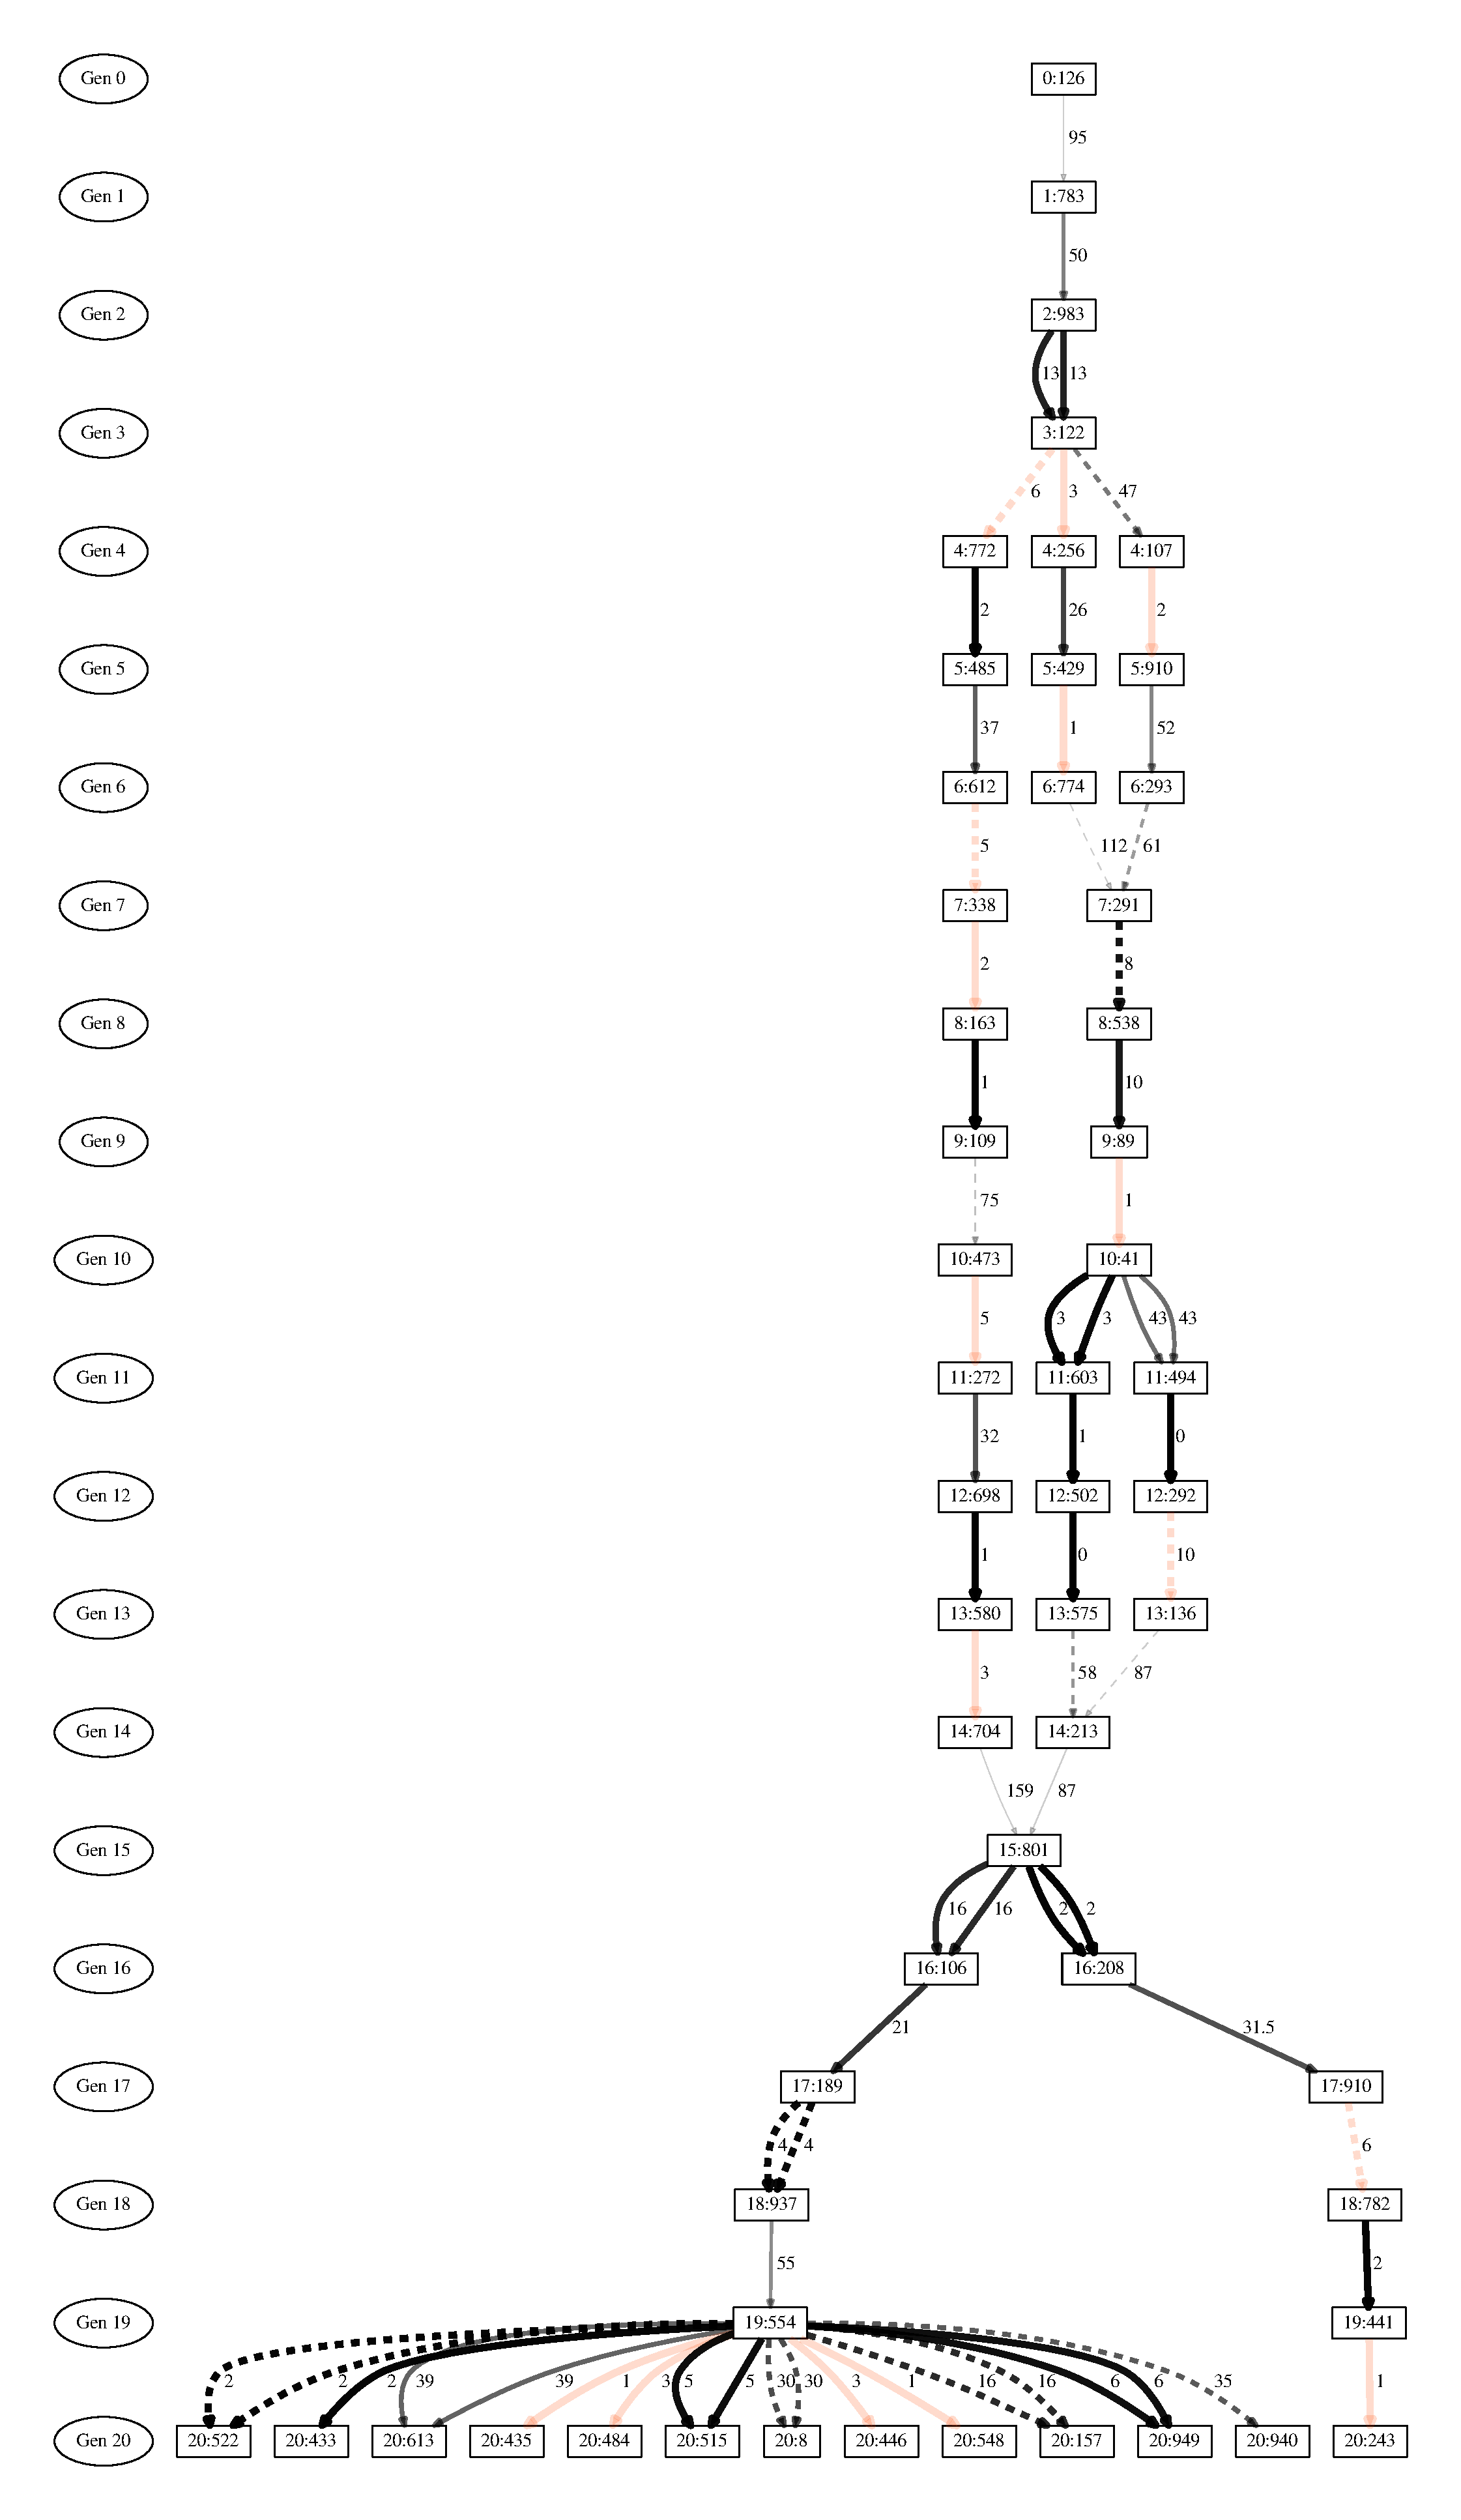
\includegraphics[width=0.9\textwidth]{../figures/run0_filtered_BandW}
	\end{center}
	\caption{The labelled run.}
	\label{fig:run0Labelled}       % Give a unique label
\end{figure}

\begin{itemize}
	\item Describe the basics of the run (length, etc.).
	\item Include at least Figure~\ref{fig:run0Labelled}, but we'll need to
	replace the orange edges with something black and white friendly. 
	Maybe also include 
	black and white versions of one or both of Figures~\ref{fig:run0full} or 
	(less likely?)~\ref{fig:run0filtered}.
	\item Talk a little about one of the final solutions (probably 20:484 or 20:548 since they differ by just one from their parent.), including the simplified solution and how/why it works.
\end{itemize}

Then work backwards from the winner back through to the start of the run.

\subsection{The (successful) end}

Figure~\ref{prog:simplified20:484} 
\todo{Should the code be in a figure, or just in-lined here in the text? I \emph{think} the figure
	will be closer to the text when more of Section 2 is written. -- NFM}
is the simplified version the successful program from 
individual 20:484. Individual 20:484's genome contains 194 genes, and the unsimplified 
program also contains 194 instructions and passes both
the training and testing cases. The simplified program in 
Figure~\ref{prog:simplified20:484} contains only 9 instructions and
also passes all the tests. 
The simplified program is actually a pretty ``human'' program, and is structured similar to 
how a person might implement replace-space-with-newline using Push. The first five 
instructions (together on the first line) replace all the spaces in the input string 
with newlines (using the \texttt{string\_replacechar} instruction) and print the 
resulting string, thereby solving half the problem. 
The next four instructions (on the second line) remove all the spaces from
a fresh copy of the input string, compute the length and leave that on the
\texttt{:integer} stack as the ``returned'' result.

\begin{figure}[h]
\begin{verbatim}
(\space \newline in1 string_replacechar print_string
 in1 \space string_removechar string_length)
\end{verbatim}
\caption{The simplified version of the successful program from individual 20:484. The
	five instructions on the first line replace all the spaces in the input string with newlines
	and print the result, solving half the problem. The next four instructions (on the second
	line) remove all the spaces from the input string and computing it's length, providing
	the desired ``returned'' result.}
\label{prog:simplified20:484}
\end{figure}

\subsection{How did we get there?}

A few places where we might need to bring in an individual that's 
missing from Figure~\ref{fig:run0Labelled}:
\begin{itemize}
	\item 19:554's other parent
	\item 17:189's other parent
	\item 12:698 and 10:473's other parents.
	\item Maybe 9:89 and 8:538's other parents. Depends somewhat on how much
	they're contributing to the final individual, and whether those 
	contributions are coming from the few changes that come from their other
	parent.
	\item Maybe 6:612, 5:429, and 4:107's other parents. (Same issues as above.)
	\item Maybe 2:983 and 1:783's other parents. If we're running long, though, 
	we could effectively start the process at 2:983 since most everything is
	pretty clean from there down.
\end{itemize}

%\caption{If the width of the figure is less than 7.8 cm use the 
%	\texttt{sidecaption} command to flush the caption on the left side of the 
%	page. If the figure is positioned at the top of the page, align the 
%	sidecaption with the top of the figure -- to achieve this you simply need 
%	to use the optional argument \texttt{[t]} with the \texttt{sidecaption} 
%	command}

\begin{figure}[tb!p] %[b] sets the image at the bottom of the page; t = top, b = bottom, h = here%
	% \sidecaption
	% Use the relevant command for your figure-insertion program
	% to insert the figure file.
	% For example, with the graphicx style use
	\begin{center}
		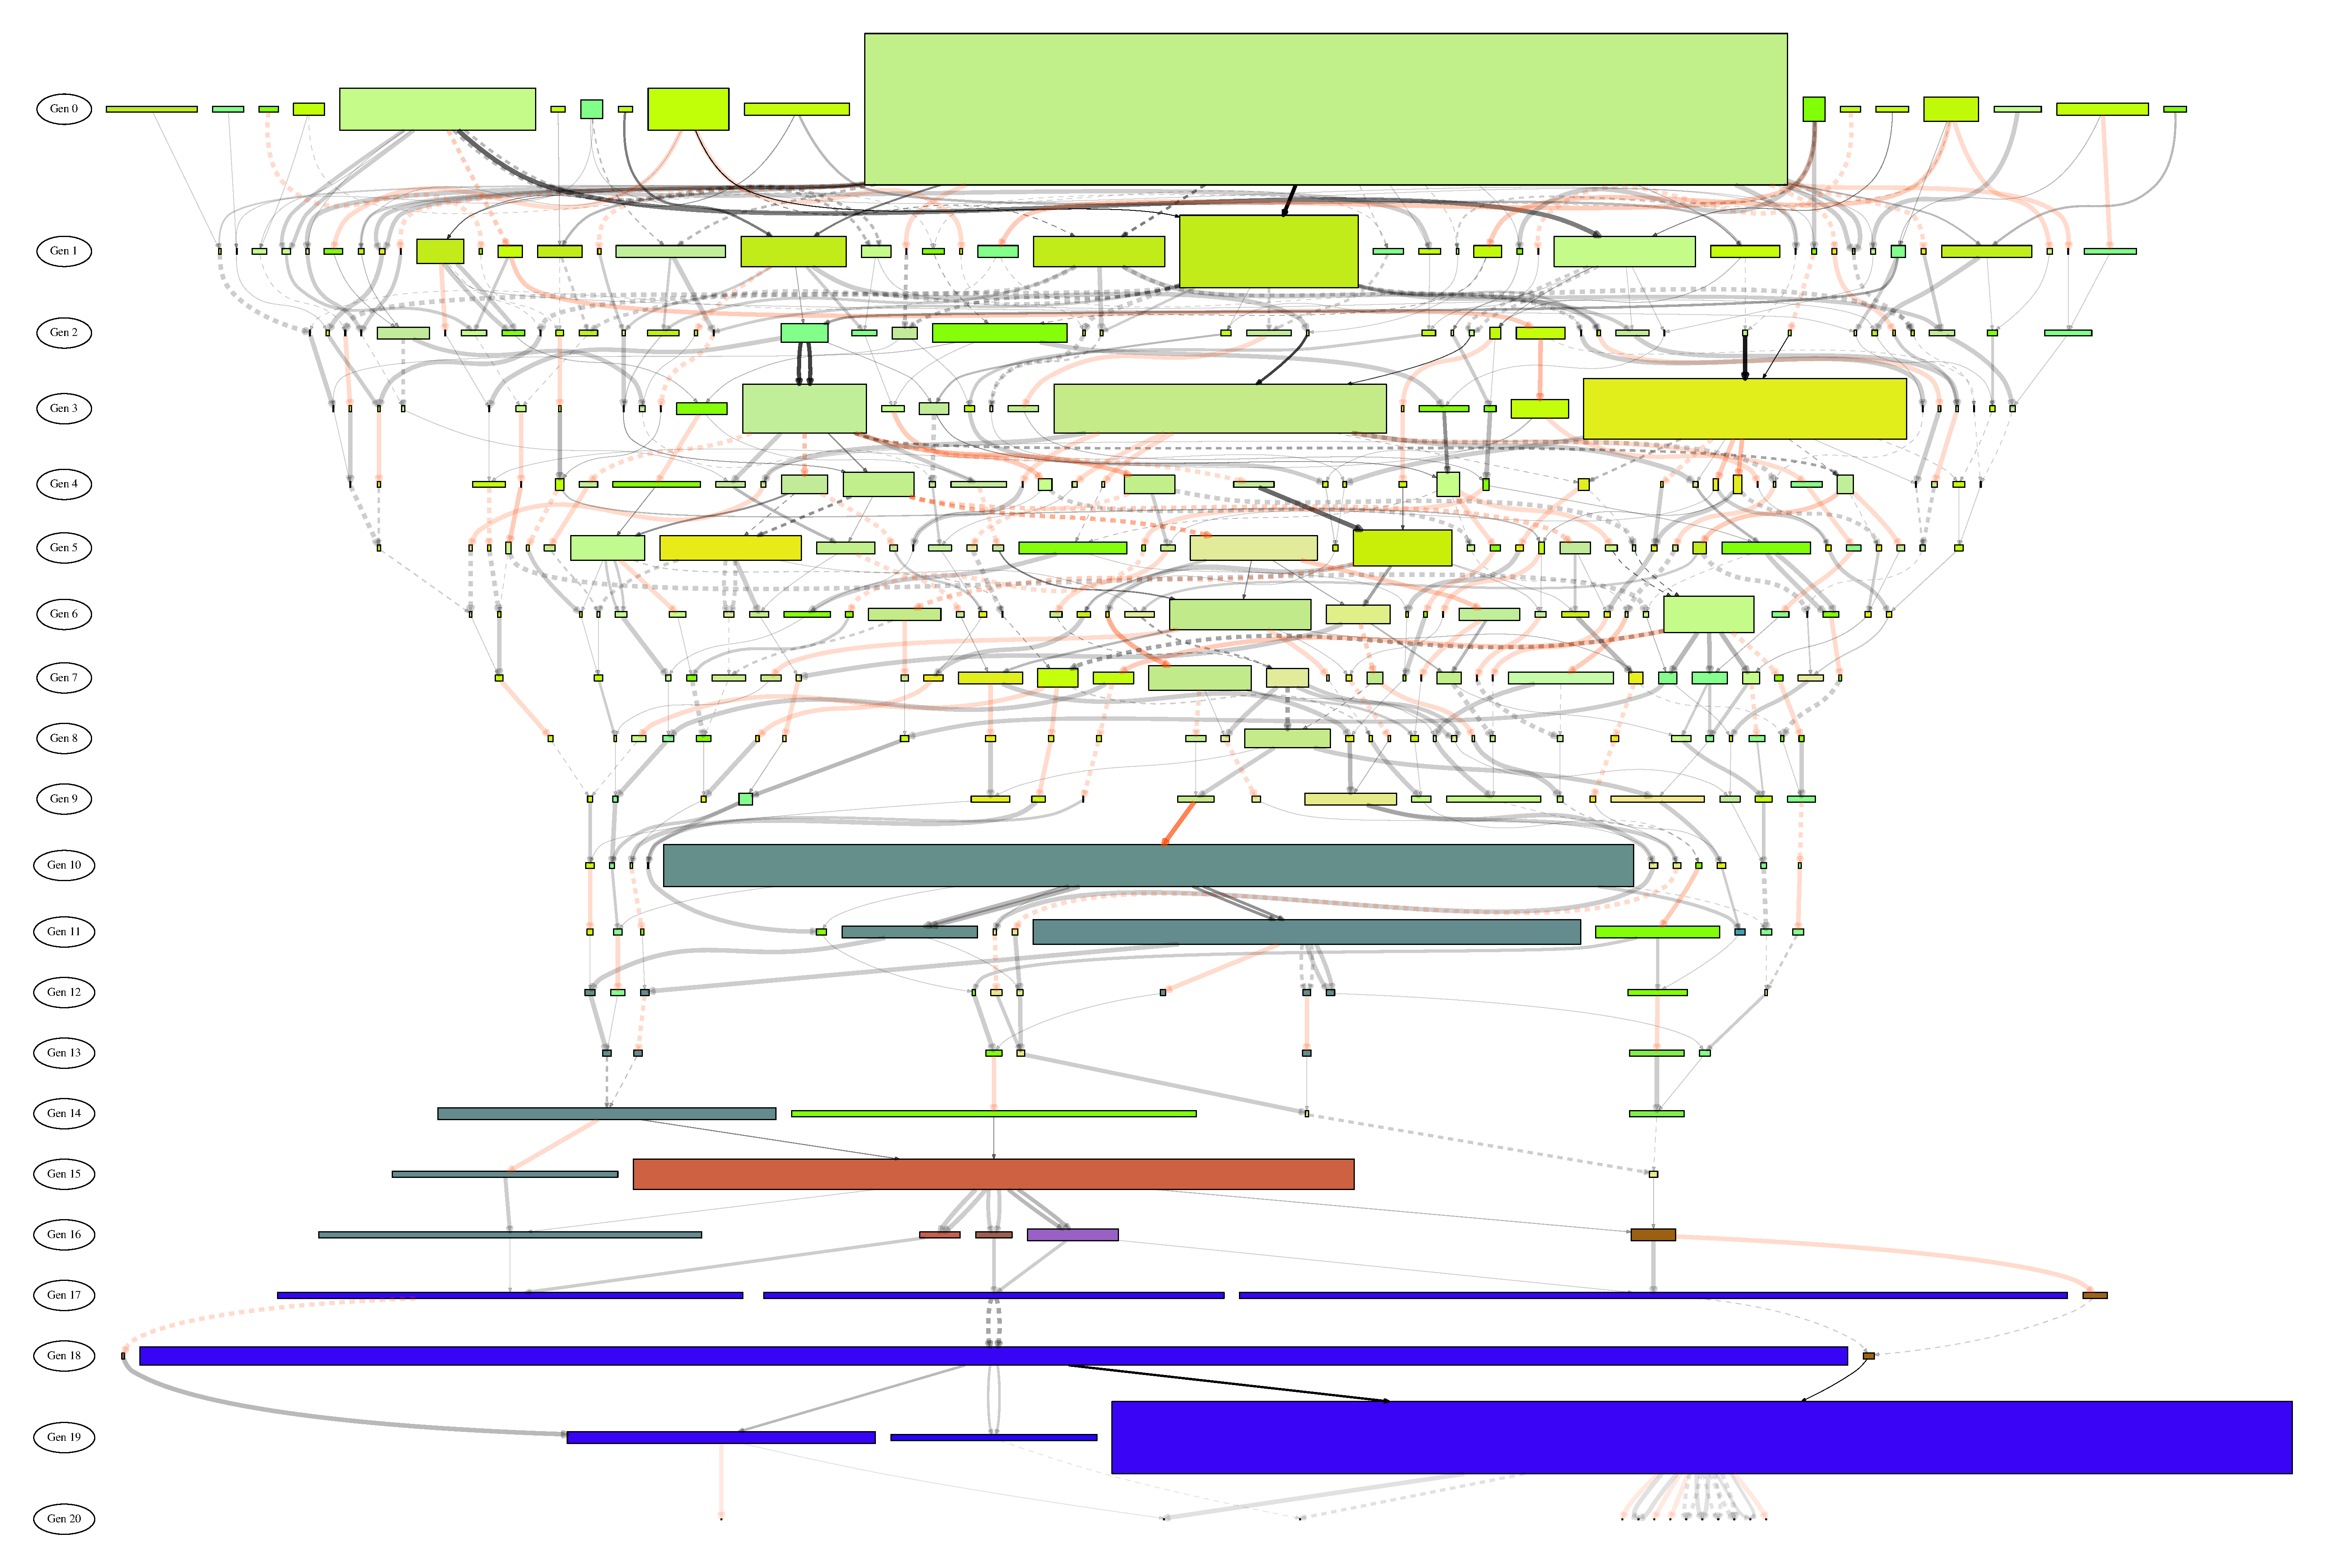
\includegraphics[width=0.9\textwidth]{../figures/run0_RBM_color_full_30000}
	\end{center}
	\caption{The full ancestry graph.}
	\label{fig:run0full}       % Give a unique label
\end{figure}

\begin{figure}[tb!p] %[b] sets the image at the bottom of the page; t = top, b = bottom, h = here%
	% \sidecaption
	% Use the relevant command for your figure-insertion program
	% to insert the figure file.
	% For example, with the graphicx style use
	\begin{center}
		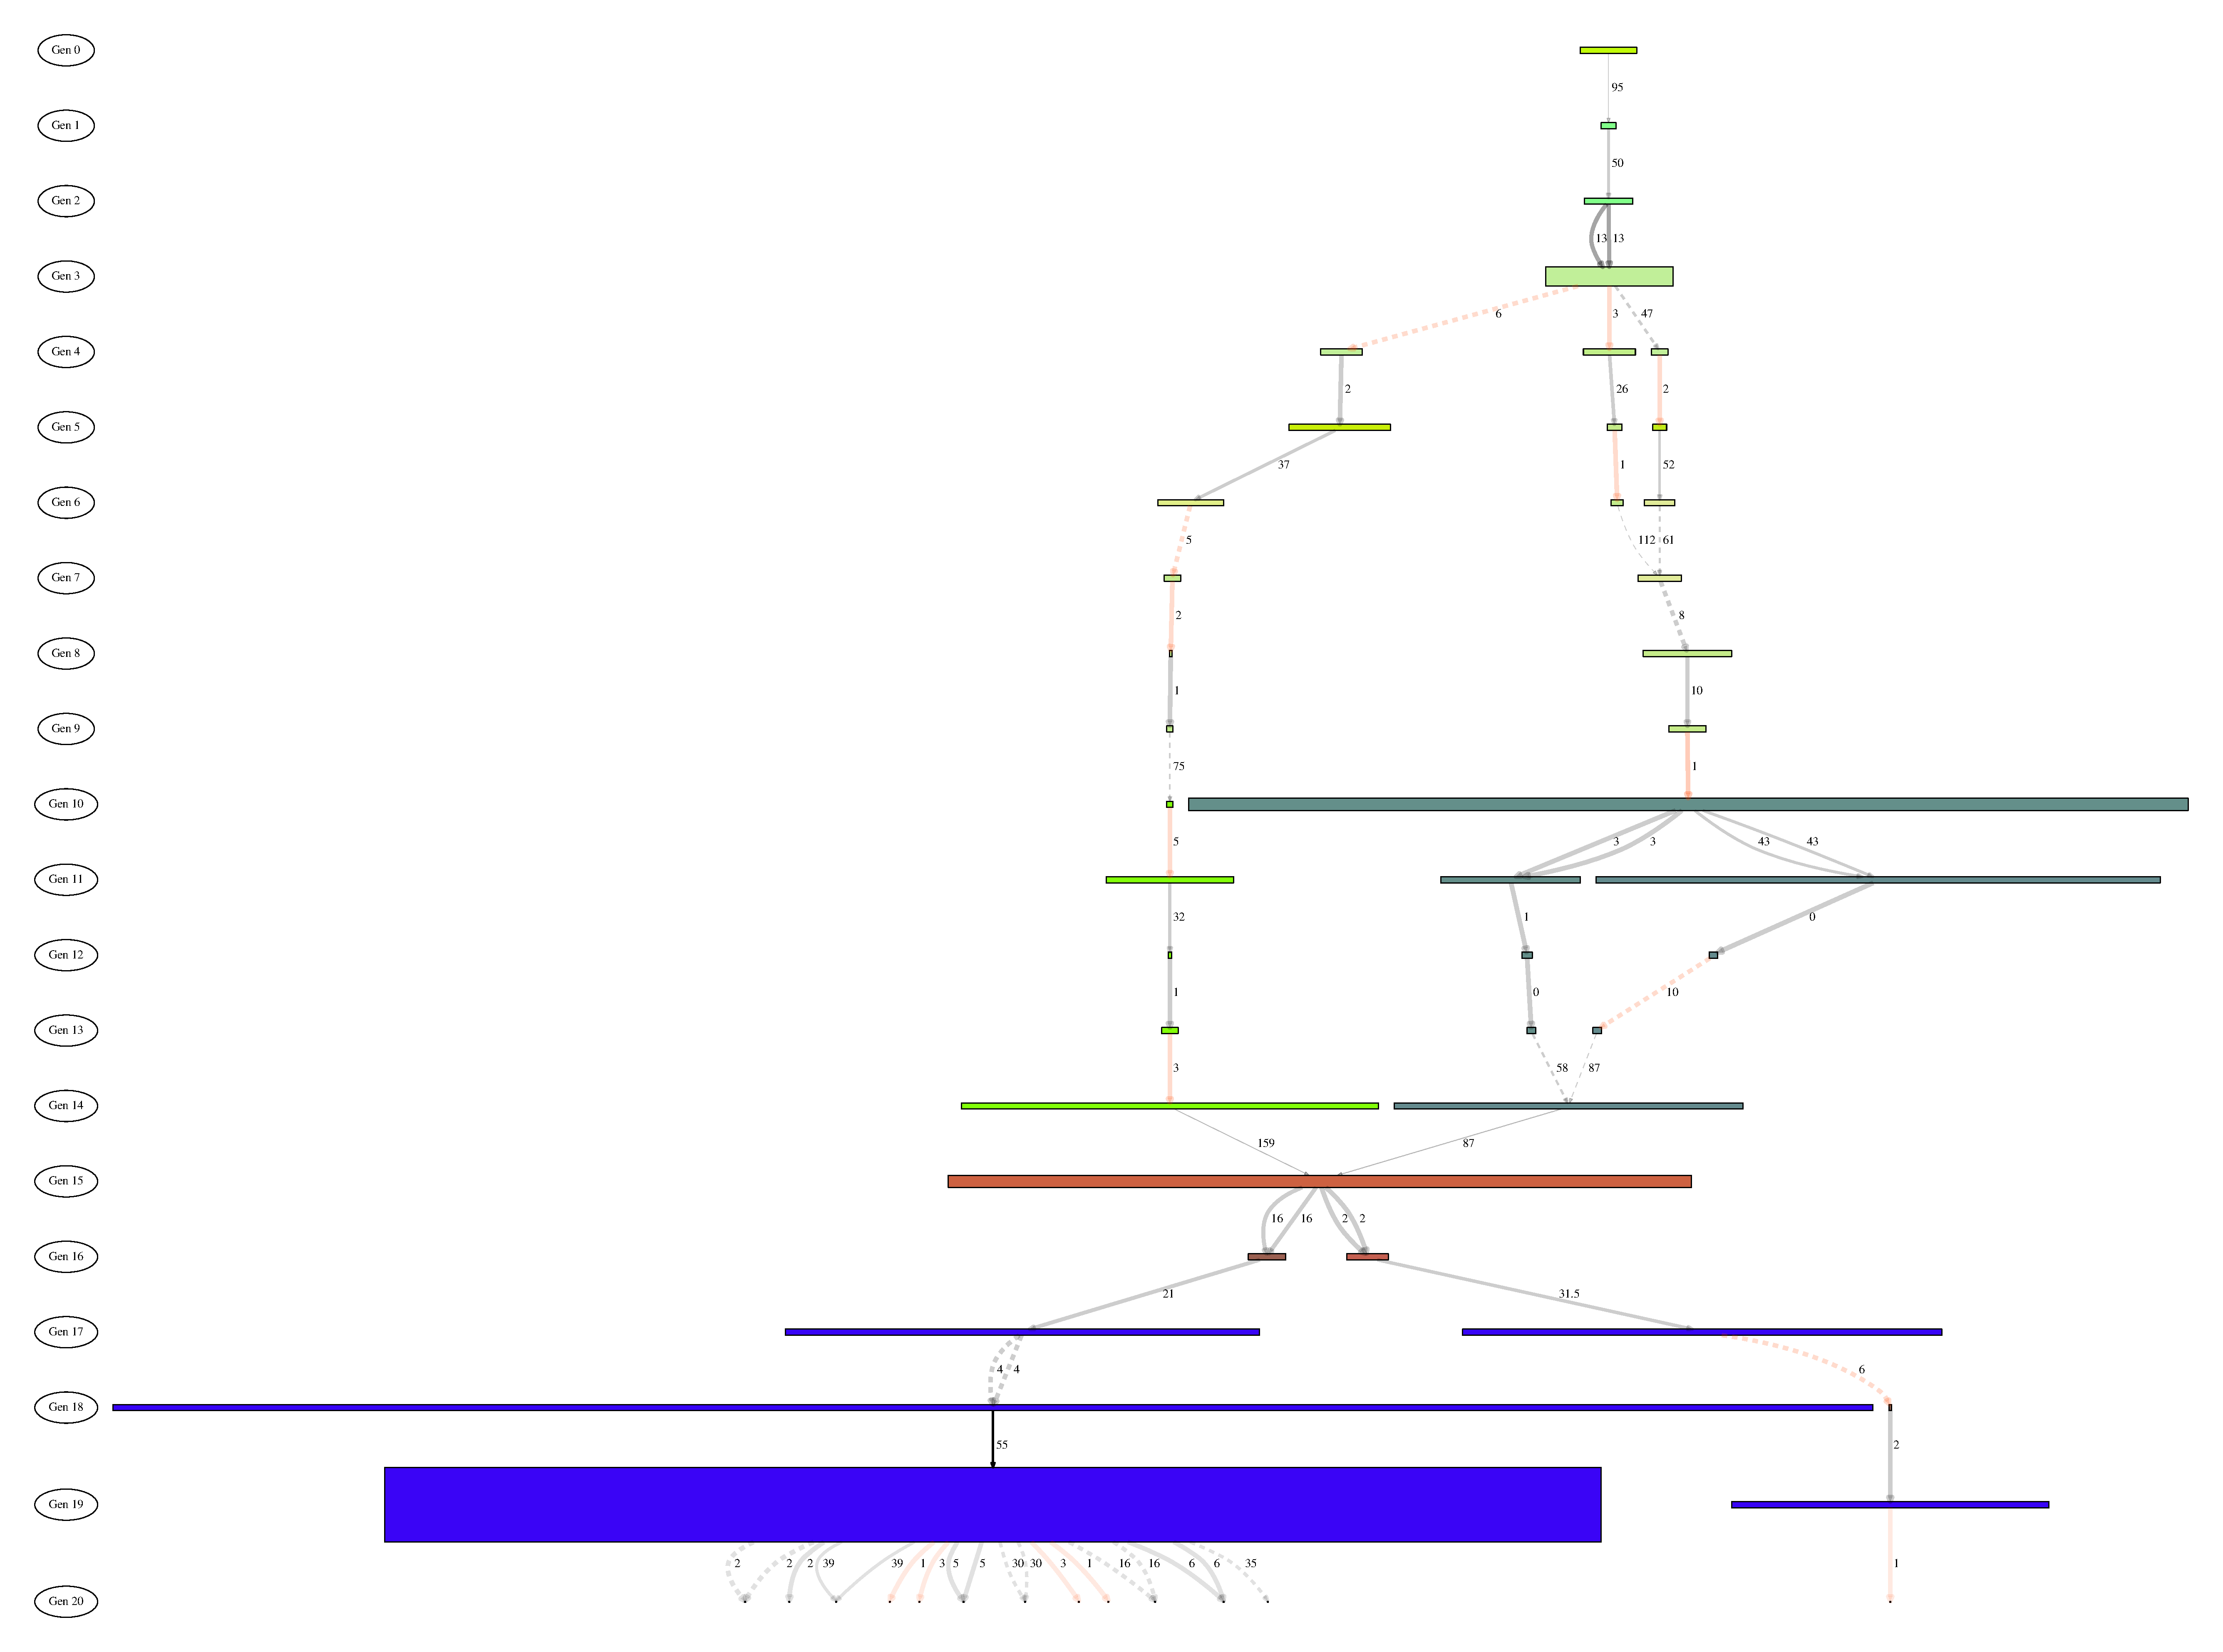
\includegraphics[width=0.9\textwidth]{../figures/run0_RBM_color_filtered_30000}
	\end{center}
	%
	% If no graphics program available, insert a blank space i.e. use
	%\picplace{5cm}{2cm} % Give the correct figure height and width in cm
	%
	\caption{The filtered ancestry graph.}
	\label{fig:run0filtered}       % Give a unique label
\end{figure}

\subsection{15:801: An important crossover}
\label{sec:15:801}

\begin{table}
\begin{tabular}{cc|cc|cc}
1 & \texttt{(\textbackslash space)} & 1 & \texttt{(\textbackslash space} & 1 & \texttt{in1} \\ 
2 & \texttt{(\textbackslash newline)} & 2 & \texttt{(\textbackslash newline)} & 2 &  \\ 
3 &  & 3 & \texttt{exec\_dup} & 3 &  \\ 
4 & \texttt{in1} & 4 & \texttt{in1} & 4 &  \\ 
5 & \texttt{string\_replacechar} & 5 & \texttt{string\_replacechar} & 5 &  \\ 
6 & \texttt{print\_string} & 6 & \texttt{print\_string} & 6 & \texttt{print\_string} \\ 
7 & \texttt{boolean\_stackdepth} & 7 & \texttt{exec\_dup} & 7 & \texttt{exec\_dup} \\ 
8 & \texttt{print\_newline} & 8 & \texttt{strin\_eq} & 8 & \texttt{exec\_s} \\ 
9 &  & 9 &  & 9 & \texttt{exec\_dup} \\ 
10 &  & 10 &  & 10 & \texttt{exec\_rot} \\ 
11 &  & 11 &  & 11 & \texttt{string\_exec string\_fromboolean} \\ 
12 &  & 12 &  & 12 & {char\_eq} \\ 
13 &  & 13 &  & 13 & \texttt{string\_emptystring boolean\_stackdepth in1 integer\_gt} \\ 
14 &  & 14 &  & 14 & \texttt{string\_emptystring} \\ 
15 &  & 15 & \texttt{(\textbackslash space)} & 15 & \texttt{(\textbackslash space)} \\ 
16 &  & 16 & \texttt{string\_dup} & 16 & \texttt{string\_dup} \\ 
17 &  & 17 & \texttt{string\_removechar} & 17 & \texttt{string\_removechar} \\ 
18 &  & 18 & \texttt{string\_rot} & 18 & \texttt{boolean\_pop} \\ 
19 &   &   &   &   & \texttt{in1} \\ 
20 &   &   &   &   & \texttt{string\_butlast} \\ 
21 &   &   &   &   & \texttt{string\_last} \\ 
22 &   &   &   &   & \texttt{string\_parse\_to\_chars} \\
23 &   &   &   &   & \texttt{exec\_when} \\ 
24 &   &   &   &   & \texttt{string\_dup} \\
25 &   &   &   &   & \texttt{string\_removechar} \\
26 &   &   & \texttt{string\_last} &   & \texttt{string\_last} \\
27 &   &   & \texttt{string\_parse\_to\_chars} &   & \texttt{string\_parse\_to\_chars} \\
28 &   &   & \texttt{string\_rot} &   & \texttt{string\_rot} \\
29 &   &   & textt{in1} &   & \texttt{in1} \\
30 &   &   & \texttt{string\_stackdepth} &   & \texttt{string\_stackdepth} \\
\end{tabular}
\end{table}

\section{Discussion}
\label{sec:discussion}

Wrap up with some kind of ``big picture'' that does things like catalogs the
\emph{kinds} of operations, their frequency, etc.


% \paragraph{Paragraph Heading} %



% \subparagraph{Subparagraph Heading} In order to avoid simply listing headings of different levels we recommend to let every heading be followed by at least a short passage of text. Use the \LaTeX\ automatism for all your cross-references and citations as has already been described in Sect.~\ref{sec:2}, see also Fig.~\ref{fig:2}.

% Use the \index{} command to code your index words
% Make sure to inlcude the indexed word inside and outside of the brackets if you want the text to show up in your paragraph:
% e.g. This book is about \index{genetic programming}genetic programming. 
% If the text is not entered outside the brackets it will appear as: This book is about .

%%
%% For tables use
%%
%\begin{table}
%\caption{Please write your table caption here}
%\label{tab:1}       % Give a unique label
%%
%% Follow this input for your own table layout
%%
%\begin{tabular}{p{2cm}p{2.4cm}p{2cm}p{4.9cm}}
%\hline\noalign{\smallskip}
%Classes & Subclass & Length & Action Mechanism  \\
%\noalign{\smallskip}\svhline\noalign{\smallskip}
%Translation & mRNA$^a$  & 22 (19--25) & Translation repression, mRNA cleavage\\
%Translation & mRNA cleavage & 21 & mRNA cleavage\\
%Translation & mRNA  & 21--22 & mRNA cleavage\\
%Translation & mRNA  & 24--26 & Histone and DNA Modification\\
%\noalign{\smallskip}\hline\noalign{\smallskip}
%\end{tabular}
%$^a$ Table foot note (with superscript)
%\end{table}

\section{Conclusions}
\label{sec:conclusions}

We did it! Yay! Oh, and it was useful and matters in some way.

\begin{acknowledgement}
	Mitchell Finzel, Emma Sax, Laverne Schrock, and Leonid Scott helped 
	with the initial computation and analyses of the differences between the 
	parents and children discussed here. William Tozier provided a host of 
	ideas and feedback all through the process.
\end{acknowledgement}

\bibliographystyle{spbasic}
\bibliography{gp-bibliography,chapter}
